\documentclass[12pt]{article}

\usepackage{enumerate}
\usepackage{graphicx}
\usepackage{geometry}
\usepackage{float}
\usepackage{appendix}
\usepackage{color}
\usepackage{amsmath}
\usepackage{pifont}
\usepackage{fancyhdr}
\usepackage{enumitem}
\usepackage{amssymb}
\usepackage{listings}

% Used to change the section number specifically
\newcommand{\mysection}[2]{\setcounter{section}{#1}\addtocounter{section}{-1}\section{Question #1}}
% \mysection{2}{Question 2}

\fancyhf{}


\geometry{a4paper}
\geometry{left = 2cm}
\geometry{right = 2cm}
\geometry{top = 3cm}
\geometry{bottom = 3cm}

\pagestyle{fancy}
\lhead{CSC236 Fall 2023}
\rhead{Problem Set 1}
\cfoot{\thepage}

\title{CSC236 Problem Set 1}

\author{Xuanqi Wei 1009353209}

\date{\today}

\begin{document}


% \maketitle
% \thispagestyle{empty}

% \newpage

% \tableofcontents
% \thispagestyle{empty}

% \newpage

\setcounter{page}{3}

% \section{Question 1}
% \begin{enumerate}[label=(\alph*)]
%     \item According to the definition of P:
%     $$\forall g_1 \in G_1,\ \exists t_1 \in T_1,\ t_1\ tiles\ g_1 \implies \forall g_2 \in G_2,\ \exists t_2 \in T_2,\ t_2\ tiles\ g_2 $$

%     \item 
%     Firstly, assume $$\forall g_1 \in G_1,\ \exists t_1 \in T_1,\ t_1\ tiles\ g\text{, which is the antecedent.}$$
    
%     Secondly, I will do the consequent part, which: $$Let\ g_2\ be\ an\ arbitrary\ element\ from\ G_2$$ 
%     Then, I want to prove that $$\exists t_2 \in T_2,\ t_2\ tiles\ g_2$$ \quad \quad \quad \quad \quad \quad \quad by selecting a satisfying element $t_2$ from $T_2$ 
%     and prove the element $t_2$ satisfies $t_2\ tiles\ g_2$.

%     \item The diagram above illustrates one instance of $G_2$ grids, which being tiled by triominoes.
    
%     Firstly, we already know that for P(1), the statement $\forall g_1 \in G_1,\ \exists t_1 \in T_1,\ t_1\ tiles\ g$ is true which is the antecedent of this direct proof.

%     Secondly, the above diagram is an element of the set of all $2^2 \times 2^2$ grid with one square removed, which is an element of $G_2$. 
%     By visulising those colorful triominoes, we see a combination triominoes, $t_2$, which is an element of the set of all tilings of elements of $G_2$ using triominoes, belonging to $T_2$, exists and tiles $g_2$.

%     Therefore, the diagram above illustrates an instance of that direct proof.

%     \item Given the statement to prove: $\forall n \in \mathbb{N},\ P(n)$, which for each natural n you can tile any $2^n \times 2^n$ grid with one cell missing using only triominoes.
    
%     \textbf{Proof:} We prove this by Simple Induction on n.


%     \textbf{Base Case:} Let $0 \leq n \leq 1$.

%     Since $G_0$ is the set of $2^0 \times 2^0$ grid with on cell removed, which $G_0$ does not contain any grid, meaning there does not exist $g_0 \in G_0$, which the statement $\forall g_0 \in G_0,\ \exists t_0 \in T_0,\ t_0\ tiles\ g_0$ is vacuously True.

%     Since $G_1$ is the set of all $2^1 \times 2^1$ grids with one cell removed, which by definition is a single triominoe.
    
%     Therefore, $\forall g_1 \in G_1,\ \exists t_1 \in T_1,\ t_1\ tiles\ g_1$ is true, which P(1) is true.

%     \textbf{Induction Step:} Let $k \in \mathbb{N}$.
    
%     \textbf{Induction Hypothesis:} Assume that $P(k)$ is true.

%     By Induction Hypothesis, we know that $P(k)$ is true, which $\forall g_k \in G_k,\ \exists t_k \in T_k,\ t_k\ tiles\ g_k $ is true.
%     I will take 3 different $g_k$s, the first with right button corner square missing, the second with right top corner square missing, and the third with left top corner square missing.
%     I will make the missing corners in these 3 $g_k$s face inwards and add a triomino which will result in getting a `L' shape.
%     The remaining $\frac{1}{4}$ place is missing a cell to form a $g_{k+1}$, which can actually be an arbitraty element from $G_k$.
%     By Induction Hypothesis, since $\forall g_k \in G_k,\ \exists t_k \in T_k,\ t_k\ tiles\ g_k $ is true, the remaining $G_k$ place can be covered by trimonoes, proving the $P(k+1)$ is true.

%     Therefore, we've proved $\forall n \in \mathbb{N},\ P(n)$ is true. 

%     $\quad \quad \quad \quad \quad \quad \quad \quad \quad \quad \quad \quad \quad \quad \quad \quad \quad \quad \quad \quad \quad \quad \quad \quad \quad \quad \quad \quad \quad \quad \quad \quad \quad \quad \quad \quad \quad \blacksquare $
% \end{enumerate}

% \newpage

\mysection{2}{Question 2}
\begin{enumerate}[label=(\alph*)]
    \item
\begin{figure*}[h]
    \centering
    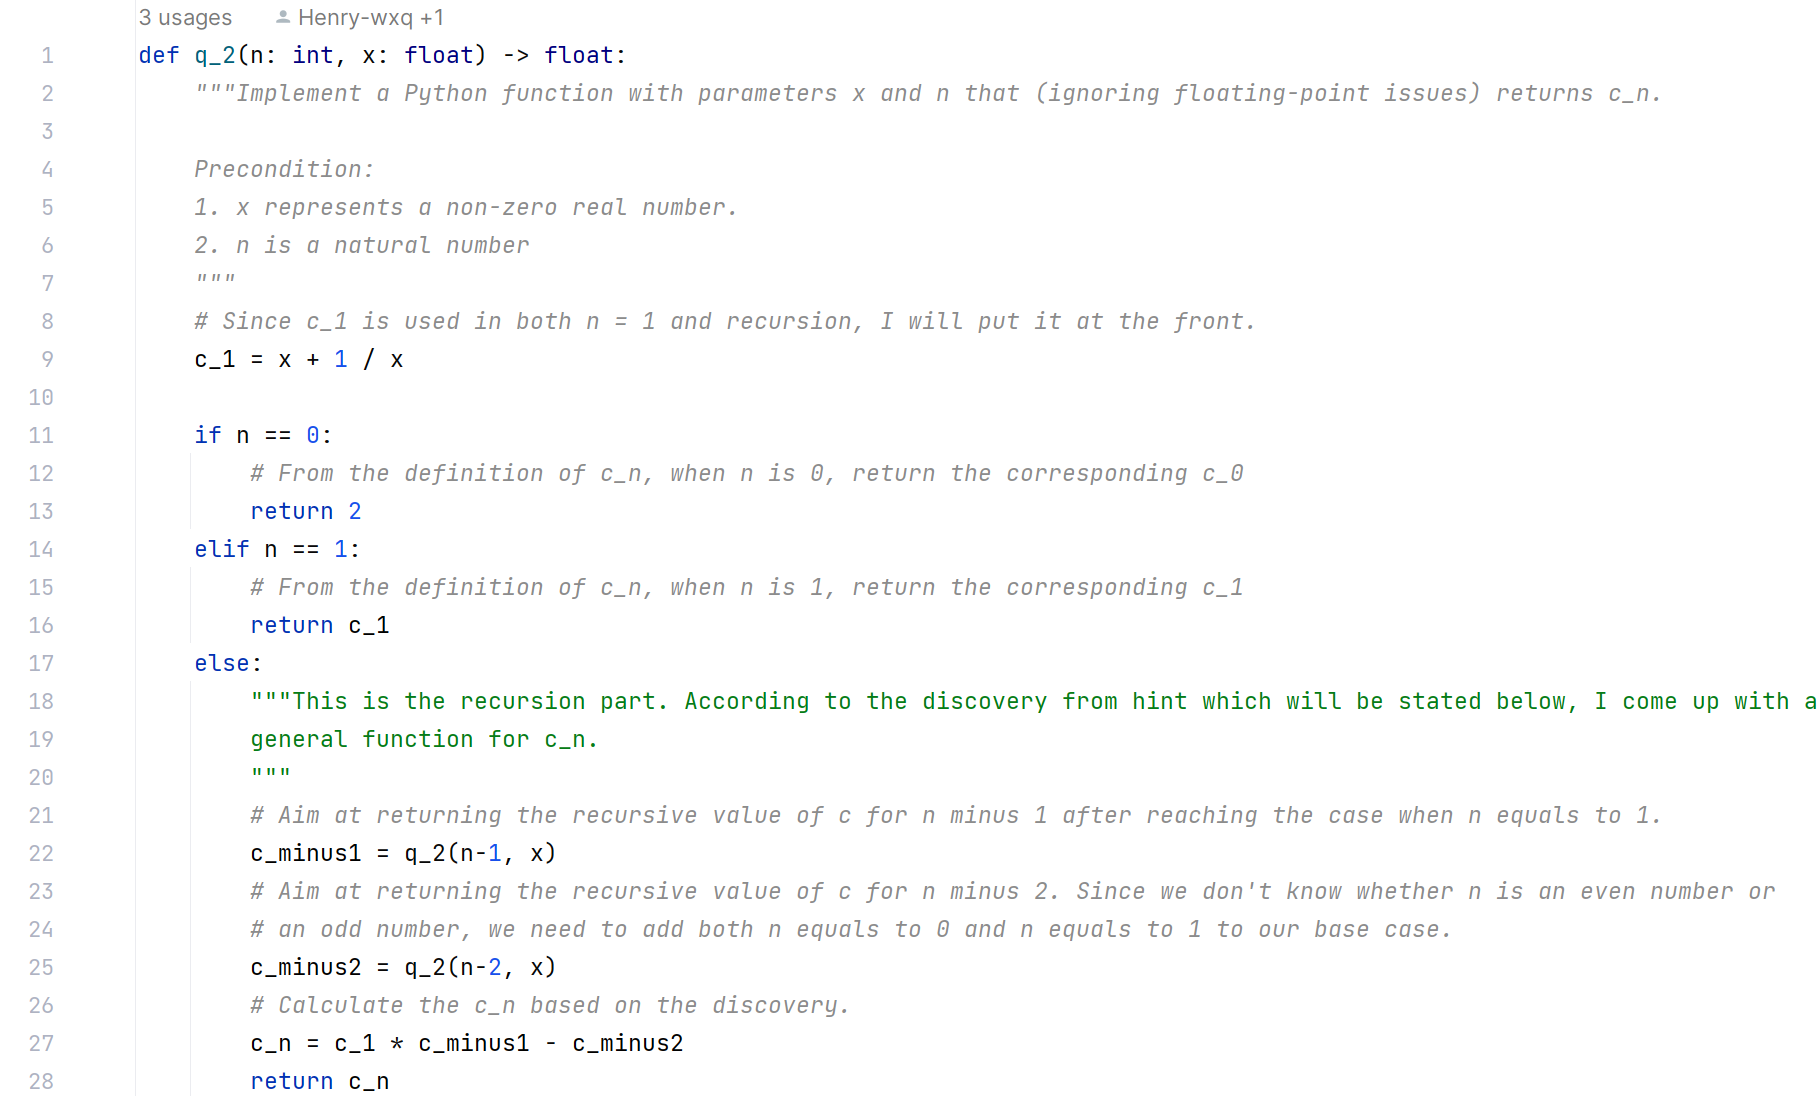
\includegraphics[width = 1.0\textwidth]{../tex_pic/q2_3.png}
    \caption{Python function for Q2-a}
\end{figure*}

\noindent The above code is the Python function with parameter x and n that (ignoring floating-point issues) returns $c_n$, the comments are both in the code above and below.

\noindent Firstly, I clearly stated the pre-conditions on x and n in a header comment, which $x \in \mathbb{R} / \{0\} $ and $n \in \mathbb{N}$.

\noindent Secondly, at line 9, I write the calculation of $c_1$ because it will be used in both `elif' statement at line 14 and `else' statement at line 17, avoiding redundancy.

\noindent Thirdly, I implemented the based case when n equals to 0 and n equals to 1 according to the definition of $c_n$.

\noindent Fourthly, I implemented the recursion based on the discovery from hint.

\begin{align*}
    (x + \frac{1}{x}) \cdot (x^n + \frac{1}{x^n}) &= x^{n+1} + \frac{1}{x^{n-1}} + x^{n-1} + \frac{1}{x^{n+1}} \\
    &= (x^{n+1} + \frac{1}{x^{n+1}}) + (x^{n-1} + \frac{1}{x^{n-1}})
\end{align*}

\noindent According to the definition of $c_n$, gives:
\begin{align*}
    c_1 \cdot c_n &= c_{n+1} + c_{n-1} \\
    \implies c_{n+1} &= c_1 \cdot c_n - c_{n-1}
\end{align*}
\noindent Thus, we generalize the above equation into: $c_{n} = c_1 \cdot c_{n-1} - c_{n-2} $, which is the core of our recursive part, at line 27.

\noindent Fifthly, aiming at returning the recursive value of $c_{n-1}$ after reaching the case when n eqials to 1, I write the code line 22.
Aiming at return the recursive value of $c_{n-2}$, I write the code at line 29.
Since we don't know whether n is an even number or an odd number, we need to add both n equals to 0 and n equals to 1 to our base case at line 11 and at line 14.

\noindent Finally, we can obtain the $c_n$ using the recursive function without use any loops, or any helper functions, nor call any exponentiation functions.

    \item To state a recurrence for the sequence c, I will start from $n=0$, which $c_0 = x^0 + \frac{1}{x^0} = 2$.
    
    Then I will goes to $n=1$, which $c_1 = x + \frac{1}{x}$.

    Moreover, for $ n\geq 2$, from the hint, we have:
    \begin{align*}
        (x + \frac{1}{x}) \cdot (x^n + \frac{1}{x^n}) &= x^{n+1} + \frac{1}{x^{n-1}} + x^{n-1} + \frac{1}{x^{n+1}} \\
        &= (x^{n+1} + \frac{1}{x^{n+1}}) + (x^{n-1} + \frac{1}{x^{n-1}})
    \end{align*}
    \noindent According to the definition of $c_n$, gives:
    \begin{align*}
        c_1 \cdot c_n &= c_{n+1} + c_{n-1} \\
        \implies c_{n+1} &= c_1 \cdot c_n - c_{n-1}
    \end{align*}

    Thus, we generalize the above equation into: $c_{n} = c_1 \cdot c_{n-1} - c_{n-2}$.

    Therefore, we have:

    $$c_n =  \left\{ \begin{array}{lcl}
        2 & \mbox{for} & n = 0 \\
        x + \frac{1}{x} & \mbox{for} & n=1 \\
        c_1 \cdot c_{n-1} - c_{n-2} & \mbox{for} & n\geq2
    \end{array}\right. $$

    \item If $x+\frac{1}{x}$ is an integer, then $x^n + \frac{1}{x^n} $ is an integer for each $n \in \mathbb{N}$
    
    Assume $x+\frac{1}{x}$ is an integer.

    Given statement to prove: $\forall n \in \mathbb{N},\ P(n)$, which $P(n)$: $x^n + \frac{1}{x^n}$ is an integer where $x \in \mathbb{R} / \{0\}$

    \textbf{Proof:} We prove this by complete induction on n.

    \textbf{Base Case:} Let $0 \leq n \leq 1$

    For $n=0$, we have $x^0 + \frac{1}{x^0} = 2$ is an integer, which P(0) is True.

    By assumption, $x + \frac{1}{x}$ is an integer, which P(1) is True.

    We've proved that $P(0)\ \&\ P(1)$ is true.

    \textbf{Induction Step:} Let $n > 1$
    
    \textbf{Induction Hypothesis:} Assume $\forall k,\ 1 \leq k < n,\ P(k)$

    WTS: $P(n)$

    From induction hypothesis, when $k_1 = 1,\ 1 \leq k_1 < n$, $P(1)$ is true, which $x + \frac{1}{x}$ is an integer.
    
    From induction hypothesis, when $k_{n-1} = n-1,\ 1 \leq k_{n-1} < n$, $P(n-1)$ is true, which $x^{n-1} + \frac{1}{x^{n-1}}$ is an integer.

    From induction hypothesis, when $k_{n-2} = n-2,\ 1 \leq k_{n-2} < n$, $P(n-2)$ is true, which $x^{n-2} + \frac{1}{x^{n-2}}$ is an integer.

    Thus, we obtain that 
    \begin{align*}
        &(x+\frac{1}{x})\cdot (x^{n-1} + \frac{1}{x^{n-1}}) - (x^{n-2} + \frac{1}{x^{n-2}})\ \text{is an integer.} \\
        =\ &x^n + \frac{1}{x^{n-2}} + x^{n-2} + \frac{1}{x^n} - x^{n-2} - \frac{1}{x^{n-2}} \\
        =\ &x^n + \frac{1}{x^n} \ \text{is an integer}
    \end{align*}

    I've proved that $P(n)$ is true.

    To conclude, I've proved that if $x+\frac{1}{x}$ is an integer, then $x^n + \frac{1}{x^n} $ is an integer for each $n \in \mathbb{N}$.

    $\quad \quad \quad \quad \quad \quad \quad \quad \quad \quad \quad \quad \quad \quad \quad \quad \quad \quad \quad \quad \quad \quad \quad \quad \quad \quad \quad \quad \quad \quad \quad \quad \quad \quad \quad \quad \quad \blacksquare $
\end{enumerate}

% \newpage

% \section{Question 3}
% (a)
% \begin{figure*}[h]
%     \centering
%     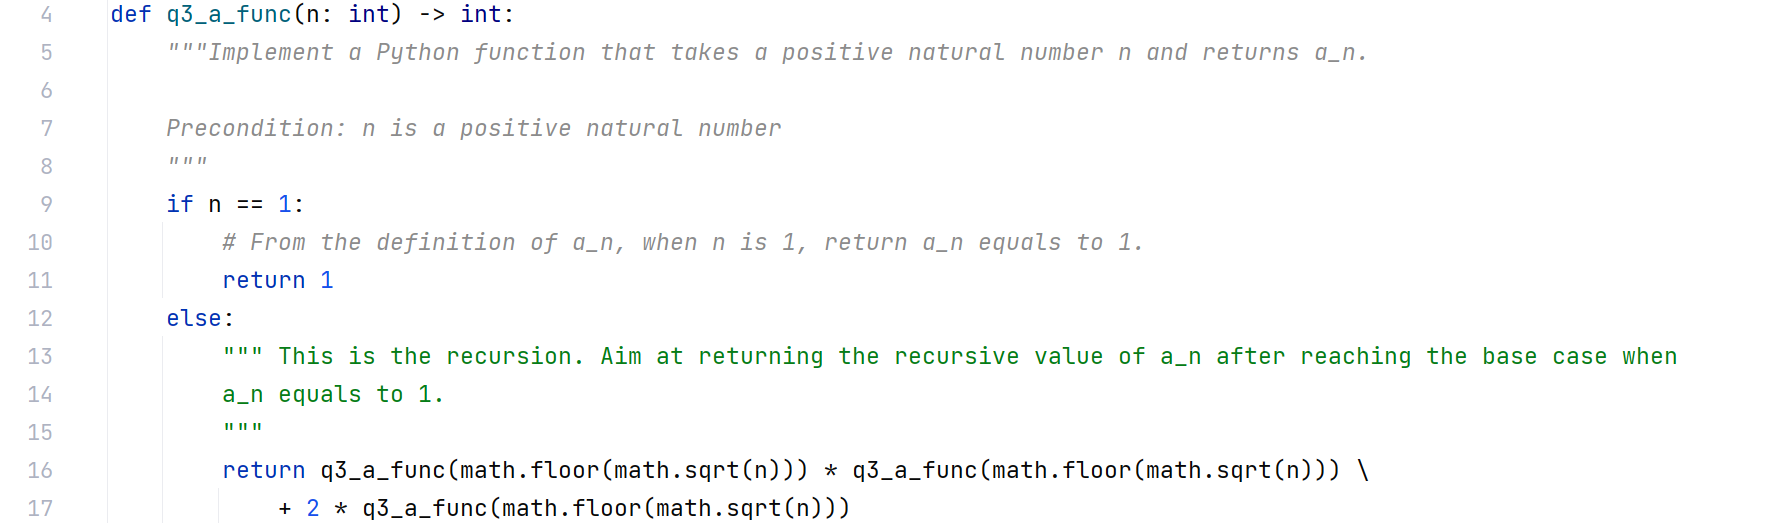
\includegraphics[width = 1.0\textwidth]{tex_pic/q3_a.png}
%     \caption{Python function for Q3-a}
% \end{figure*}

% \noindent (b)
% \begin{figure*}[h]
%     \centering
%     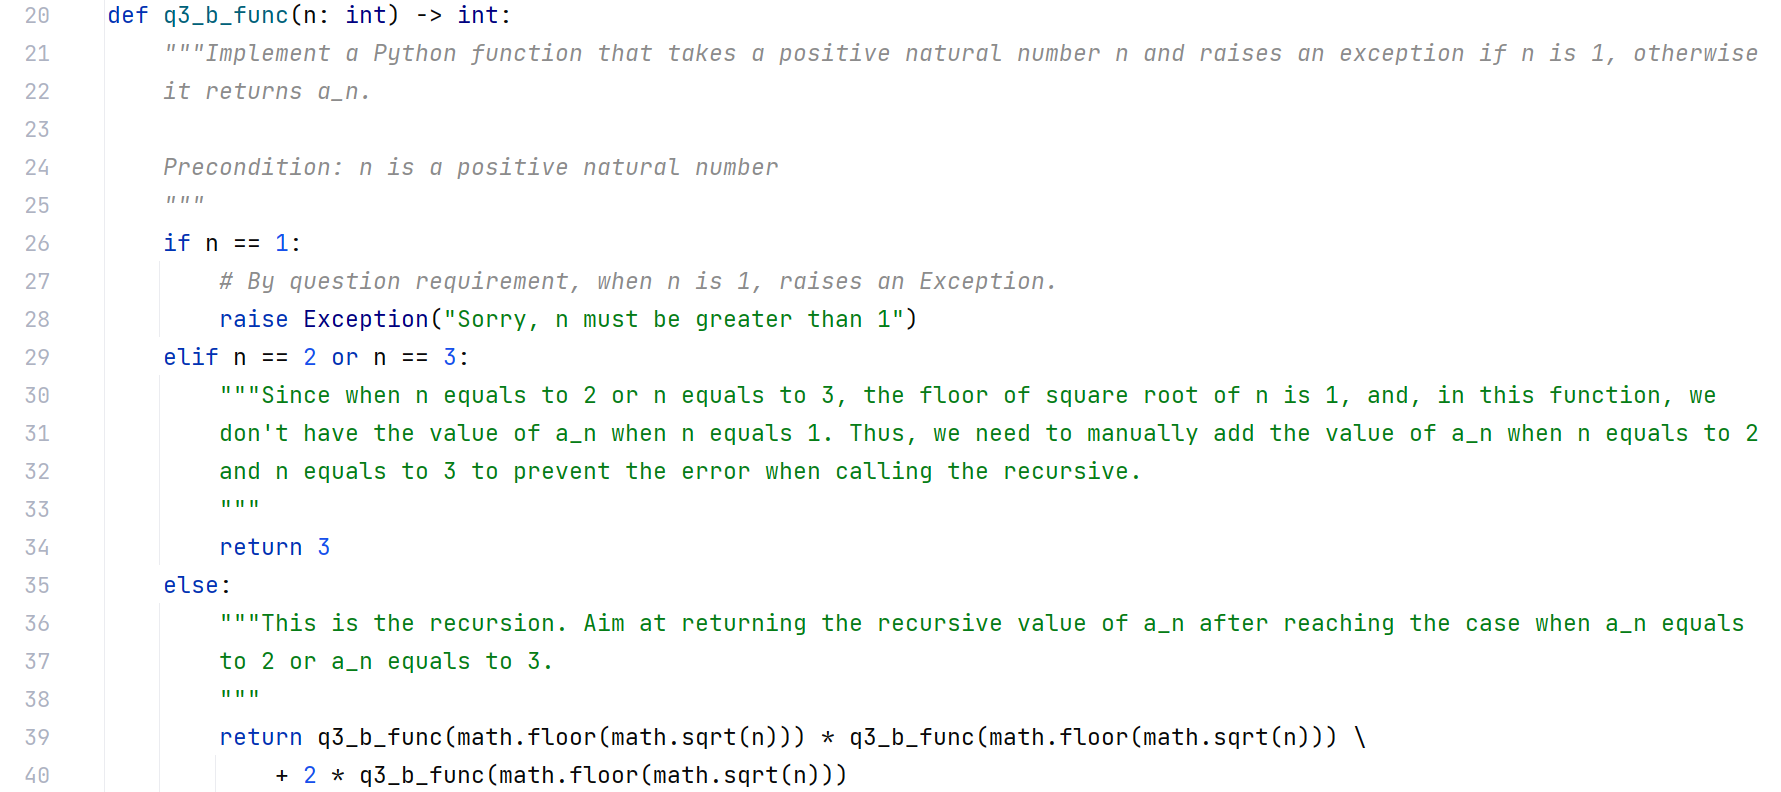
\includegraphics[width = 1.0\textwidth]{tex_pic/q3_b.png}
%     \caption{Python function for Q3-b}
% \end{figure*}

% \begin{enumerate}[label=(\alph*)]
% \setcounter{enumi}{2}
%     \item When $n_0 = 2$, $n_0$ is the smallest natural $n_0$ so that $a_n$ is a multiple of 3 for each natural $ n \geq n_0$.
    
%     Given statement to prove: $\forall n \in \mathbb{N},\ n \geq n_0,\ P(n)$, which $P(n):$ $a_n$ is a multiple of 3.

%     Let $n \in \mathbb{N}$.

%     \textbf{Proof:} We prove this by complete induction on n.

%     \textbf{Base Case:} Let $2 \leq n < 4$.
%     \begin{align*}
%         P(2):\ a_2 &= (a_{\lfloor \sqrt{2} \rfloor})^2 + 2 \cdot a_{\lfloor \sqrt{2} \rfloor} \\
%         &= a_1^2 + 2 \cdot a_1 = 1^2 + 2 = 3 \text{is a multiple of 3}.
%     \end{align*}
%     \begin{align*}
%         P(3):\ a_3 &= (a_{\lfloor \sqrt{3} \rfloor})^2 + 2 \cdot a_{\lfloor \sqrt{3} \rfloor} \\
%         &= a_1^2 + 2 \cdot a_1 = 1^2 + 2 = 3 \text{is a multiple of 3}.
%     \end{align*}

%     Thus, I've proved the base case is true.

%     \textbf{Induction Step:} Let $n \geq 4$.

%     \textbf{Induction Hypothesis:} Assume $\forall k,\ 2\leq k < n,\ P(k)$

%     Since $n \geq 4$, gives $\lfloor \sqrt{n} \rfloor < n$.

%     Since $\lfloor \sqrt{n} \rfloor < n$ and $4 \leq n$, gives $2 \leq \lfloor \sqrt{n} \rfloor$ as 2 is the smallest value of $\lfloor \sqrt{n} \rfloor$, which gives, $$2 \leq \lfloor \sqrt{n} \rfloor < n $$

%     Since $\lfloor \sqrt{n} \rfloor$ is an integer which $\lfloor \sqrt{n} \rfloor \geq 2$, from induction hypothesis, we can always find $k' = \lfloor \sqrt{n} \rfloor$, which $P(k')$ is true and $a_{k'} = 3p,\ p \in \mathbb{N}$.

%     Thus gives,
%     \begin{align*}
%         a_n &= (\lfloor \sqrt{n} \rfloor)^2 + 2\cdot a_{\lfloor \sqrt{n} \rfloor} \\
%         &= (a_{k'})^2 + 2\cdot a_{k'} \\
%         &= (3p)^2 + 2 \cdot (3 \cdot p) \\
%         &= 9 \cdot p^2 + 6 \cdot p \\
%         &= 3 \cdot (3\cdot p^2 + 2p)
%     \end{align*}

%     Let $q=3\cdot p^2 + 2\cdot p$.
%     Since $p \in \mathbb{N}$, gives $q \in \mathbb{N}$, which $$a_n = 3q,\ q \in \mathbb{N}\ \text{, where $a_n$ is a multiple of 3.}$$
%     I've proved that $P(n)$ is true.

%     To conclude, I've proved when $n_0 = 2$, $n_0$ is the smallest natural $n_0$ so that $a_n$ is a multiple of 3 for each natural $ n \geq n_0$.

%     $\quad \quad \quad \quad \quad \quad \quad \quad \quad \quad \quad \quad \quad \quad \quad \quad \quad \quad \quad \quad \quad \quad \quad \quad \quad \quad \quad \quad \quad \quad \quad \quad \quad \quad \quad \quad \quad \blacksquare $
% \end{enumerate}


\end{document}